\documentclass{article}
\usepackage{graphicx}
\usepackage{hyperref}
\usepackage{caption}
\usepackage{subcaption}
\usepackage[dutch]{babel}

\begin{document}

\begin{center}
	\huge{Wiskunde in Kunst}\\
	\LARGE{Opdracht 4} \\
	
	\vspace{2cm}
	
	\Large{Chaostheorie}\\
	
	\vfill
	
	\begin{figure}[Hh]
		\centering
		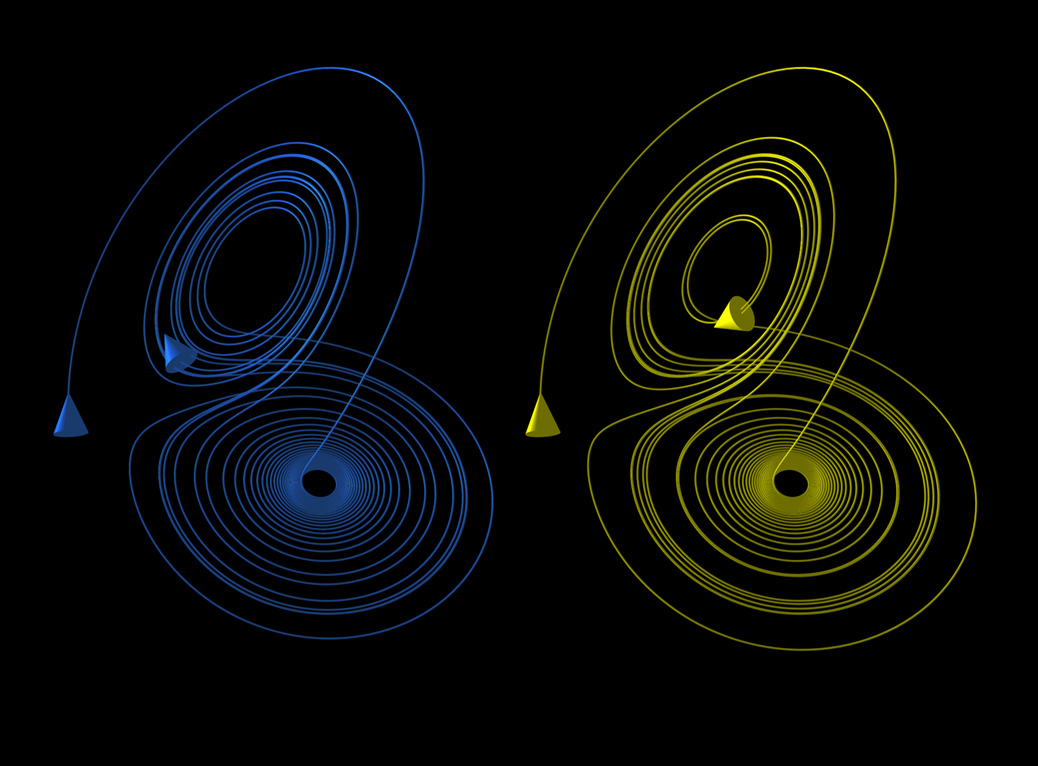
\includegraphics[width=\textwidth]{TwoLorenzOrbits}
		\label{}
	\end{figure}
	
	\vfill
	\Large{Marcelo Dias Avelino} \hfill \large{0840416}
\end{center}

\pagebreak

\section{Wat is de chaostheorie?}

De chaostheorie is een wiskundig gebied waarin het gedrag van bepaalde dynamische systemen worden onderzocht. 

Een dynamische systeem is een systeem met geheugen en het gedrag van het systeem wordt volledig door wat er in het geheugen zit en door de invloed van de omgeving bepaald. Het geheugen heet de `toestand' van het systeem en het wordt beschreven met getallen. Dit soort systemen zijn onderverdeeld in zo genaamd orde systemen. Dit betekent dat bij een eerste-ordersysteem het geheugen maar \'e\'en stap ver gaat, twee stappen bij een tweede-ordersysteem, enzovoort. Een voorbeeld van een eerste-ordersysteem is een leeglopend bad; het enige stap dat het neemt is het leeglopen van het water. Dit kan beschreven worden met \'e\'en getal: hoe snel het leegloopt. Een tweede-ordesysteem neemt, zoals eerder uitgelegd, twee stappen en is daarom beschreven door twee getallen. Een bekende voorbeeld van zo een systeem is een gewicht die op een veer rust. De twee stappen zijn dan de snelheid van het gewicht en de uitrekking van de veer. Dit soort systemen kunnen van heel simpel, zoals het voorbeeld van de bad, tot onmogelijk complex gaan, zoals hoeveel zalmen aanwezig zijn in een meer tijdens de lente. 

Deze systemen zijn puur deterministisch, dat betekent dat het mogelijk is om uit te rekenen wat hun toestand is op een bepaalde punt maar ze zijn compleet afhankelijk van hun begin toestand. Hierdoor maken kleine verschillen in de begintoestand, zoals bijvoorbeel het afronden van getallen tijdens het uitrekenen, het voorspellen van zulke systemen in het algemeen onmogelijk. Dit gedrag staat bekend als \textit{`deterministiche chaos'}, of gewoon \textit{`chaos'} in het algemeen. 

De chaostheorie is gebaseerd op meerdere principes:

\begin{itemize}

	\item{\textbf{Het vlindereffect} \\
		Dit is het effect waarbij het flapperen van een vlinder's vleugels uiteindelijk een tornado aan de andere kant van de wereld zou kunnen veroorzaken. Het kan heel lang duren voordat het gebeurt, maar als de vlinder niet op de juist tijd en plek zijn vleugels had geflapperd, dan was de tornado er misschien nooit geweest. 

		\begin{figure}[Hh]
			\centering
			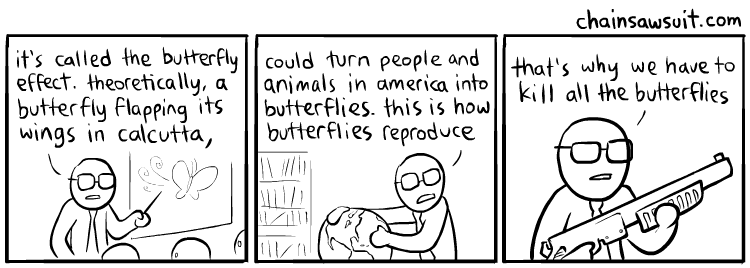
\includegraphics[width=0.8\textwidth]{butterfly-effect.png}
			\caption{Het vlindereffect uitgelegd.}
		\end{figure}

		Meerdere kleine dergelijk gebeurtenissen kunnen, als een domino-effect, een steeds grotere gebeurtenis veroorzaken. Dit is ook van toepassing op ons eigen levens; wie weet wat voor effect een kleine beslissing vandaag zal hebben in de toekomst?
	}

	\item{\textbf{Onvoorspelbaarheid} \\
		Zoals boven uitgelegd, omdat wij nooit de begintoestanden in perfecte detail kunnen weten, is het onmogelijk om de staat van een dergelijke systeem in de toekomst te voorspellen. Elke kleine fout in het meten van de begin toestanden van zo'n systeem kan tot gigantische fouten tijdens het voorspellen, in dezelfde wijze als de vlinder hierboven genoemd. We kunnen niet het effect van alle vlinders in de wereld meten en daarom blijft het juist voorspellen van het weer heel lastig.
	}

	\item{\textbf{Orde/wanorde} \\
		Chaos bestaat niet volledig alleen uit wanorde, al zou het zou wel kunnen lijken. Chaos is juist het verkennen van de transities tussen orde en wanorde.
	}

	\item{\textbf{Menging} \\
		Dit betekent dat twee punten, of bijvoorbeeld twee water moleculen, dat in het begin zich naast elkaar bevonden uiteindelijk heel ver van elkaar terecht zullen komen. De twee water moleculen zijn misschien ooit begonnen in dezelfde rivier maar kunnen uiteindelijk aan tegenovergestelde kanten van de wereld terecht komen. Dit gebeurt door turbulentie veroorzakt door andere systemen. In het geval van de moleculen zou het wind of een boot kunnen zijn geweest.

		\begin{figure}[Hh]
			\centering
			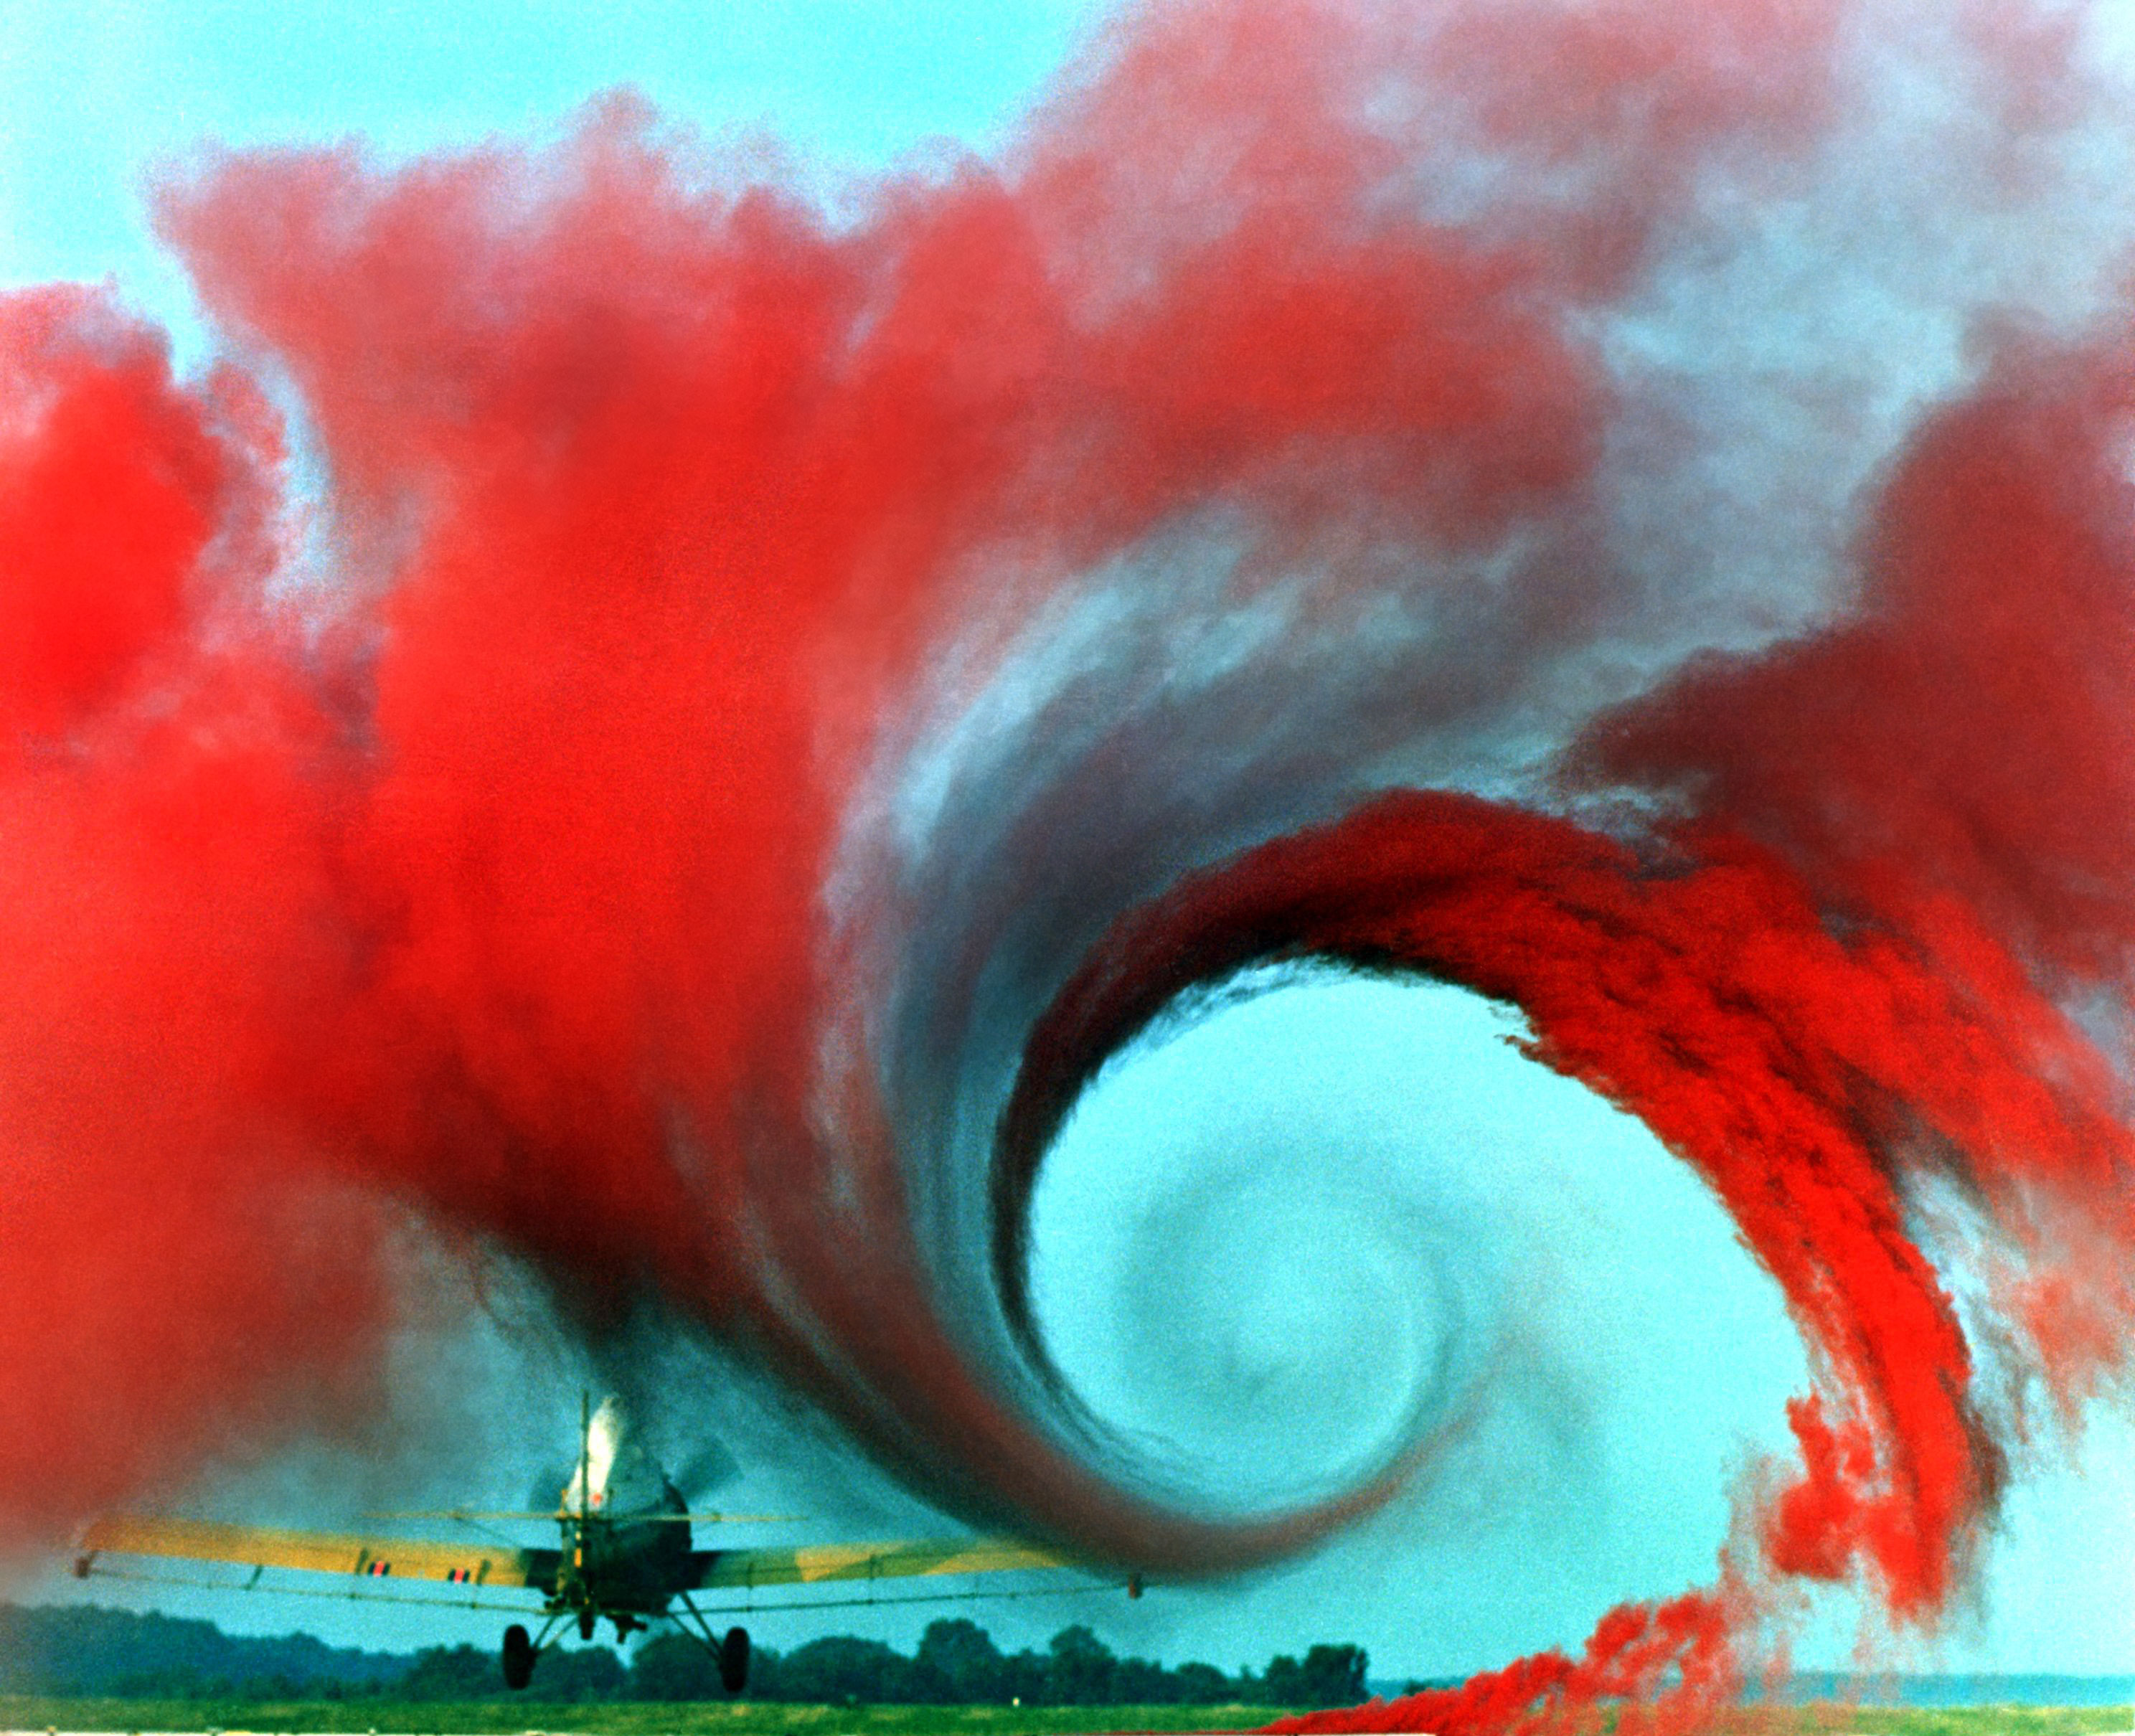
\includegraphics[width=0.5\textwidth]{Airplane_vortex}
			\caption{Menging ontstaan door turbulentie van de vliegtuig.}
		\end{figure}
	}

	\item{\textbf{Feedback} \\
		Dit heeft betrekking op reacties op elke actie die plaatsvindt. Bijvoorbeeld als de prijs van een beurs plotselling zakt, zullen de aandelen worden verkocht om zo min mogelijk geld te verliezen. Hierdoor zouden de prijzen van de aandelen weer kunnen stijgen of juist veel sneller zakken.
	}

	\item{\textbf{Fractals} \\
		Een fractal is een eindeloos patroon. Het zijn oneindig complexe patronen dat gelijksoortig zijn op meerdere schalen. Ze worden gecr\"eerd door een simpele proces steeds te herhalen in een lopend feedback loop. Ze worden gedreven door recursie, het aanroepen van zichzelf, en zijn afbeelding van dynamische systemen, ook bekend als fotos van chaos. Deze patronen komen heel vaak voor in de natuur; bomen, wolken, schelpen, etc. zijn uitgebouwd uit de soort patronen.

		\begin{figure}[Hh]
			\centering
			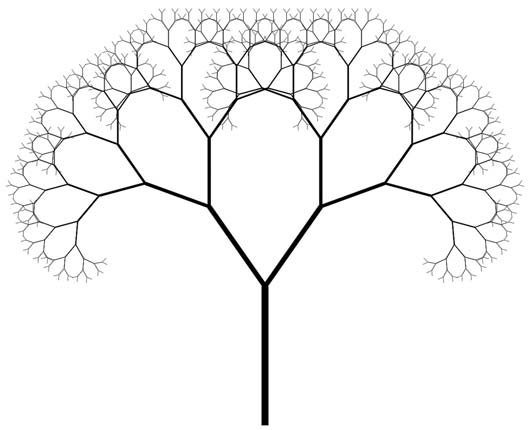
\includegraphics[width=0.5\textwidth]{fractal-tree}
			\caption{Voorbeeld van fractals in de natuur.}
		\end{figure}

	}

	\section{Het begin van het heelal}

	Met het onderzoeken van de chaostheorie, is er ook een alternatief voor de oerknal theorie onstaan, de zogenaamd \textit{Chaotische inflatie theorie}. Deze theorie probeert te bewijzen dat het helaal niet \'e\'en enkele gebeurtenis is en dat het wel begonnen is met een gigantisch knal, dat onze heelal niet het enige heelal, maar in plaats daarvan is het \'e\'en van een oneindig parallele heelals. Deze theorie is nog niet onbewezen en er is zelfs wat bewijs gevonden in de vorm van energie fluctuaties in het heelal. Dit zou kunnen uitleggen waar het heelal nou precies van is onstaan, iets wat de oerknal theorie niet kan bewijzen.

\end{itemize}

\pagebreak

\begin{thebibliography}{9}

\bibitem{}
	\url{http://en.wikipedia.org/wiki/Circle_Limit_III}
	
\end{thebibliography}

\end{document}
